% Options for packages loaded elsewhere
\PassOptionsToPackage{unicode}{hyperref}
\PassOptionsToPackage{hyphens}{url}
%
\documentclass[
]{book}
\usepackage{amsmath,amssymb}
\usepackage{lmodern}
\usepackage{iftex}
\ifPDFTeX
  \usepackage[T1]{fontenc}
  \usepackage[utf8]{inputenc}
  \usepackage{textcomp} % provide euro and other symbols
\else % if luatex or xetex
  \usepackage{unicode-math}
  \defaultfontfeatures{Scale=MatchLowercase}
  \defaultfontfeatures[\rmfamily]{Ligatures=TeX,Scale=1}
\fi
% Use upquote if available, for straight quotes in verbatim environments
\IfFileExists{upquote.sty}{\usepackage{upquote}}{}
\IfFileExists{microtype.sty}{% use microtype if available
  \usepackage[]{microtype}
  \UseMicrotypeSet[protrusion]{basicmath} % disable protrusion for tt fonts
}{}
\makeatletter
\@ifundefined{KOMAClassName}{% if non-KOMA class
  \IfFileExists{parskip.sty}{%
    \usepackage{parskip}
  }{% else
    \setlength{\parindent}{0pt}
    \setlength{\parskip}{6pt plus 2pt minus 1pt}}
}{% if KOMA class
  \KOMAoptions{parskip=half}}
\makeatother
\usepackage{xcolor}
\usepackage{color}
\usepackage{fancyvrb}
\newcommand{\VerbBar}{|}
\newcommand{\VERB}{\Verb[commandchars=\\\{\}]}
\DefineVerbatimEnvironment{Highlighting}{Verbatim}{commandchars=\\\{\}}
% Add ',fontsize=\small' for more characters per line
\usepackage{framed}
\definecolor{shadecolor}{RGB}{248,248,248}
\newenvironment{Shaded}{\begin{snugshade}}{\end{snugshade}}
\newcommand{\AlertTok}[1]{\textcolor[rgb]{0.94,0.16,0.16}{#1}}
\newcommand{\AnnotationTok}[1]{\textcolor[rgb]{0.56,0.35,0.01}{\textbf{\textit{#1}}}}
\newcommand{\AttributeTok}[1]{\textcolor[rgb]{0.77,0.63,0.00}{#1}}
\newcommand{\BaseNTok}[1]{\textcolor[rgb]{0.00,0.00,0.81}{#1}}
\newcommand{\BuiltInTok}[1]{#1}
\newcommand{\CharTok}[1]{\textcolor[rgb]{0.31,0.60,0.02}{#1}}
\newcommand{\CommentTok}[1]{\textcolor[rgb]{0.56,0.35,0.01}{\textit{#1}}}
\newcommand{\CommentVarTok}[1]{\textcolor[rgb]{0.56,0.35,0.01}{\textbf{\textit{#1}}}}
\newcommand{\ConstantTok}[1]{\textcolor[rgb]{0.00,0.00,0.00}{#1}}
\newcommand{\ControlFlowTok}[1]{\textcolor[rgb]{0.13,0.29,0.53}{\textbf{#1}}}
\newcommand{\DataTypeTok}[1]{\textcolor[rgb]{0.13,0.29,0.53}{#1}}
\newcommand{\DecValTok}[1]{\textcolor[rgb]{0.00,0.00,0.81}{#1}}
\newcommand{\DocumentationTok}[1]{\textcolor[rgb]{0.56,0.35,0.01}{\textbf{\textit{#1}}}}
\newcommand{\ErrorTok}[1]{\textcolor[rgb]{0.64,0.00,0.00}{\textbf{#1}}}
\newcommand{\ExtensionTok}[1]{#1}
\newcommand{\FloatTok}[1]{\textcolor[rgb]{0.00,0.00,0.81}{#1}}
\newcommand{\FunctionTok}[1]{\textcolor[rgb]{0.00,0.00,0.00}{#1}}
\newcommand{\ImportTok}[1]{#1}
\newcommand{\InformationTok}[1]{\textcolor[rgb]{0.56,0.35,0.01}{\textbf{\textit{#1}}}}
\newcommand{\KeywordTok}[1]{\textcolor[rgb]{0.13,0.29,0.53}{\textbf{#1}}}
\newcommand{\NormalTok}[1]{#1}
\newcommand{\OperatorTok}[1]{\textcolor[rgb]{0.81,0.36,0.00}{\textbf{#1}}}
\newcommand{\OtherTok}[1]{\textcolor[rgb]{0.56,0.35,0.01}{#1}}
\newcommand{\PreprocessorTok}[1]{\textcolor[rgb]{0.56,0.35,0.01}{\textit{#1}}}
\newcommand{\RegionMarkerTok}[1]{#1}
\newcommand{\SpecialCharTok}[1]{\textcolor[rgb]{0.00,0.00,0.00}{#1}}
\newcommand{\SpecialStringTok}[1]{\textcolor[rgb]{0.31,0.60,0.02}{#1}}
\newcommand{\StringTok}[1]{\textcolor[rgb]{0.31,0.60,0.02}{#1}}
\newcommand{\VariableTok}[1]{\textcolor[rgb]{0.00,0.00,0.00}{#1}}
\newcommand{\VerbatimStringTok}[1]{\textcolor[rgb]{0.31,0.60,0.02}{#1}}
\newcommand{\WarningTok}[1]{\textcolor[rgb]{0.56,0.35,0.01}{\textbf{\textit{#1}}}}
\usepackage{longtable,booktabs,array}
\usepackage{calc} % for calculating minipage widths
% Correct order of tables after \paragraph or \subparagraph
\usepackage{etoolbox}
\makeatletter
\patchcmd\longtable{\par}{\if@noskipsec\mbox{}\fi\par}{}{}
\makeatother
% Allow footnotes in longtable head/foot
\IfFileExists{footnotehyper.sty}{\usepackage{footnotehyper}}{\usepackage{footnote}}
\makesavenoteenv{longtable}
\usepackage{graphicx}
\makeatletter
\def\maxwidth{\ifdim\Gin@nat@width>\linewidth\linewidth\else\Gin@nat@width\fi}
\def\maxheight{\ifdim\Gin@nat@height>\textheight\textheight\else\Gin@nat@height\fi}
\makeatother
% Scale images if necessary, so that they will not overflow the page
% margins by default, and it is still possible to overwrite the defaults
% using explicit options in \includegraphics[width, height, ...]{}
\setkeys{Gin}{width=\maxwidth,height=\maxheight,keepaspectratio}
% Set default figure placement to htbp
\makeatletter
\def\fps@figure{htbp}
\makeatother
\setlength{\emergencystretch}{3em} % prevent overfull lines
\providecommand{\tightlist}{%
  \setlength{\itemsep}{0pt}\setlength{\parskip}{0pt}}
\setcounter{secnumdepth}{5}
\usepackage{booktabs}
\ifLuaTeX
  \usepackage{selnolig}  % disable illegal ligatures
\fi
\usepackage[]{natbib}
\bibliographystyle{plainnat}
\IfFileExists{bookmark.sty}{\usepackage{bookmark}}{\usepackage{hyperref}}
\IfFileExists{xurl.sty}{\usepackage{xurl}}{} % add URL line breaks if available
\urlstyle{same} % disable monospaced font for URLs
\hypersetup{
  pdftitle={04\_trainingdata},
  pdfauthor={Casey Menick},
  hidelinks,
  pdfcreator={LaTeX via pandoc}}

\title{04\_trainingdata}
\author{Casey Menick}
\date{2022-11-20}

\begin{document}
\maketitle

{
\setcounter{tocdepth}{1}
\tableofcontents
}
\hypertarget{about}{%
\chapter{About}\label{about}}

\begin{Shaded}
\begin{Highlighting}[]
\NormalTok{bookdown}\SpecialCharTok{::}\FunctionTok{serve\_book}\NormalTok{()}
\end{Highlighting}
\end{Shaded}

\hypertarget{fire-selection}{%
\chapter{Fire Selection}\label{fire-selection}}

\hypertarget{set-up}{%
\section{Set Up}\label{set-up}}

\hypertarget{libraries}{%
\subsection{Libraries}\label{libraries}}

\begin{Shaded}
\begin{Highlighting}[]
\FunctionTok{library}\NormalTok{(tidyverse)}
\FunctionTok{library}\NormalTok{(terra)}
\FunctionTok{library}\NormalTok{(sf)}
\FunctionTok{library}\NormalTok{(mapview)}
\FunctionTok{library}\NormalTok{(raster)}
\FunctionTok{library}\NormalTok{(rgeos)}
\FunctionTok{library}\NormalTok{(lubridate)}
\FunctionTok{library}\NormalTok{(ggplot2)}
\FunctionTok{library}\NormalTok{(exactextractr)}
\FunctionTok{library}\NormalTok{(patchwoRk)}
\FunctionTok{library}\NormalTok{(gridExtra)}
\end{Highlighting}
\end{Shaded}

\hypertarget{usda-national-forest-type-group-dataset}{%
\subsection{USDA National Forest Type Group Dataset}\label{usda-national-forest-type-group-dataset}}

Conifer Forest Type Groups: Douglas-Fir, Fir-Spruce-Mountain Hemlock, Lodgepole Pine

\begin{Shaded}
\begin{Highlighting}[]
\CommentTok{\# forest type groups and key}
\NormalTok{conus\_forestgroup }\OtherTok{\textless{}{-}} \FunctionTok{raster}\NormalTok{(}\StringTok{\textquotesingle{}data/forest\_type/conus\_forestgroup.tif\textquotesingle{}}\NormalTok{)}
\NormalTok{forest\_codes }\OtherTok{\textless{}{-}} \FunctionTok{read\_csv}\NormalTok{(}\StringTok{\textquotesingle{}data/forest\_type/forestgroupcodes.csv\textquotesingle{}}\NormalTok{)}

\CommentTok{\# set crs}
\NormalTok{crs }\OtherTok{=} \FunctionTok{crs}\NormalTok{(conus\_forestgroup)}
\end{Highlighting}
\end{Shaded}

\hypertarget{epa-level-3-ecoregions}{%
\subsection{EPA level-3 Ecoregions}\label{epa-level-3-ecoregions}}

Canadian Rockies, Idaho Batholith, Middle Rockies, Columbian Mountains - Northern Rockies

\begin{Shaded}
\begin{Highlighting}[]
\CommentTok{\# level 3 ecoregions}
\NormalTok{l3eco }\OtherTok{\textless{}{-}} \FunctionTok{st\_read}\NormalTok{(}\StringTok{\textquotesingle{}data/ecoregion/us\_eco\_l3.shp\textquotesingle{}}\NormalTok{) }\SpecialCharTok{\%\textgreater{}\%} 
  \FunctionTok{st\_transform}\NormalTok{(., }\AttributeTok{crs=}\NormalTok{crs)}

\CommentTok{\# select northern rocky mountains from level3 ecoregions}
\NormalTok{eco\_select }\OtherTok{\textless{}{-}}\NormalTok{ l3eco }\SpecialCharTok{\%\textgreater{}\%} 
  \FunctionTok{filter}\NormalTok{(NA\_L3NAME }\SpecialCharTok{\%in\%} \FunctionTok{c}\NormalTok{(}\StringTok{\textquotesingle{}Canadian Rockies\textquotesingle{}}\NormalTok{,}\StringTok{\textquotesingle{}Columbia Mountains/Northern Rockies\textquotesingle{}}\NormalTok{,}\StringTok{\textquotesingle{}Middle Rockies\textquotesingle{}}\NormalTok{,}\StringTok{\textquotesingle{}Idaho Batholith\textquotesingle{}}\NormalTok{))}
\end{Highlighting}
\end{Shaded}

\hypertarget{mapping}{%
\subsection{Mapping}\label{mapping}}

\hypertarget{ecoregions}{%
\subsubsection{Ecoregions}\label{ecoregions}}

\begin{Shaded}
\begin{Highlighting}[]
\FunctionTok{mapview}\NormalTok{(eco\_select)}
\end{Highlighting}
\end{Shaded}

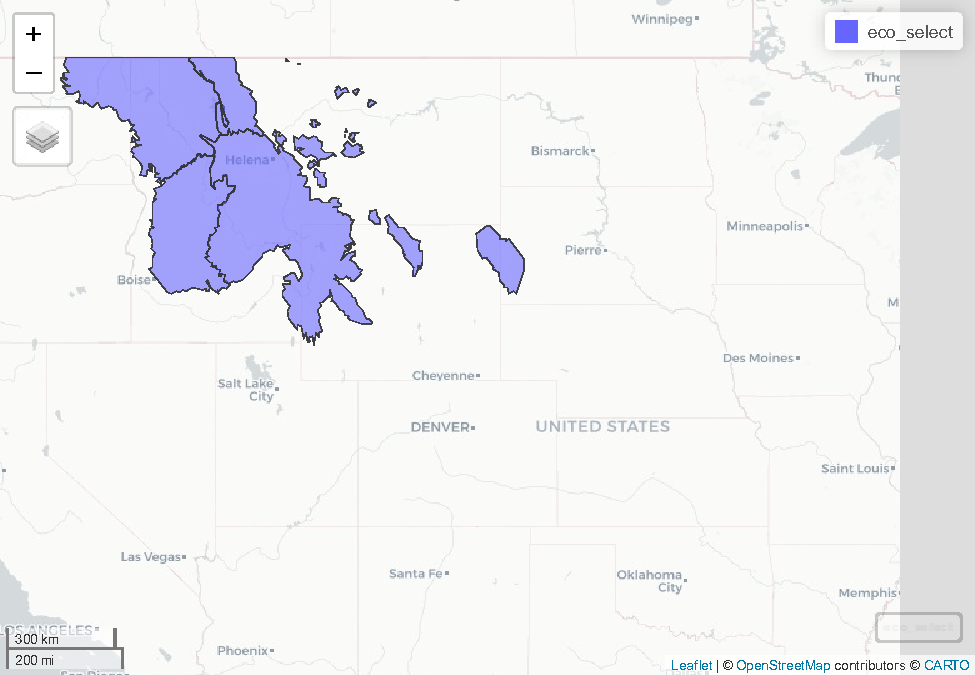
\includegraphics{_main_files/figure-latex/mapping ecoregion-1.pdf}

\hypertarget{forest-type-groups}{%
\subsubsection{Forest Type Groups}\label{forest-type-groups}}

\begin{Shaded}
\begin{Highlighting}[]
\NormalTok{forestgroup\_crop }\OtherTok{\textless{}{-}} \FunctionTok{crop}\NormalTok{(conus\_forestgroup,l3eco)}
\FunctionTok{mapview}\NormalTok{(forestgroup\_crop)}
\end{Highlighting}
\end{Shaded}

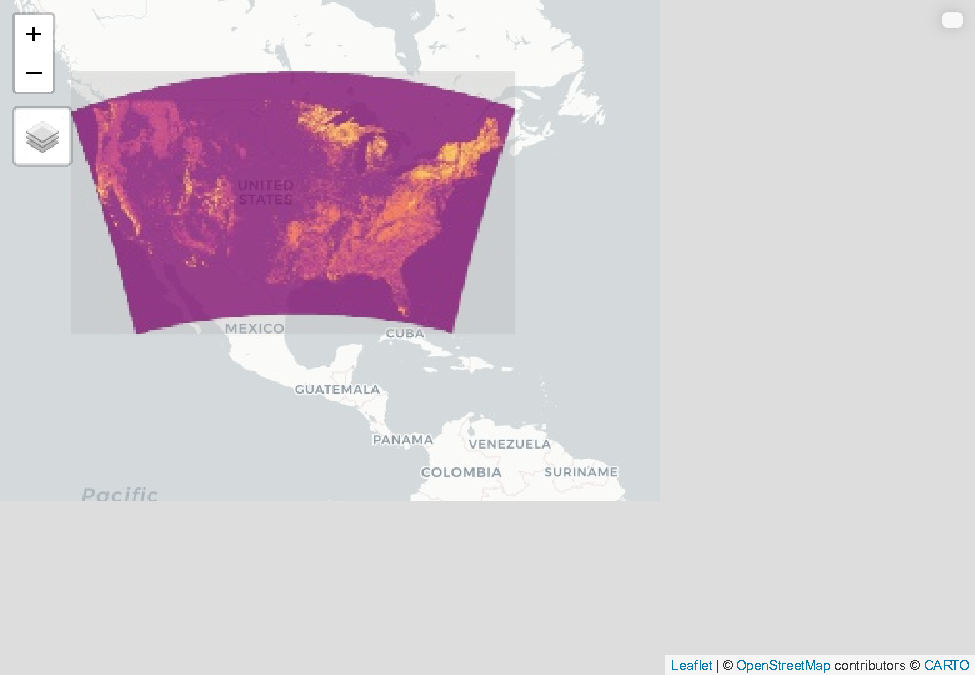
\includegraphics{_main_files/figure-latex/mapping ftype-1.pdf}

\hypertarget{define-fire-parameters}{%
\section{Define Fire Parameters}\label{define-fire-parameters}}

\hypertarget{monitoring-trends-in-burn-severity-mtbs-dataset}{%
\subsection{Monitoring Trends in Burn Severity (MTBS) Dataset}\label{monitoring-trends-in-burn-severity-mtbs-dataset}}

Criteria:

-1988-1991

-500+ acres of high-severity

-Within selected ecoregions

-\textgreater25\% of selected forest types

\begin{Shaded}
\begin{Highlighting}[]
\CommentTok{\# mtbs fire perimeters}
\NormalTok{mtbs\_full }\OtherTok{\textless{}{-}} \FunctionTok{st\_read}\NormalTok{(}\StringTok{\textquotesingle{}data/mtbs/mtbs\_perims\_DD.shp\textquotesingle{}}\NormalTok{) }\SpecialCharTok{\%\textgreater{}\%} 
  \FunctionTok{st\_transform}\NormalTok{(., }\AttributeTok{crs=}\NormalTok{crs)}

\NormalTok{mtbs\_select }\OtherTok{\textless{}{-}}\NormalTok{ mtbs\_full }\SpecialCharTok{\%\textgreater{}\%} 
  \FunctionTok{mutate}\NormalTok{(}\AttributeTok{state =} \FunctionTok{str\_sub}\NormalTok{(Event\_ID,}\DecValTok{0}\NormalTok{,}\DecValTok{2}\NormalTok{),}
         \AttributeTok{year =} \FunctionTok{year}\NormalTok{(}\FunctionTok{as.Date}\NormalTok{(Ig\_Date))) }\SpecialCharTok{\%\textgreater{}\%} 
  \FunctionTok{filter}\NormalTok{(state }\SpecialCharTok{\%in\%} \FunctionTok{c}\NormalTok{(}\StringTok{"WA"}\NormalTok{,}\StringTok{"ID"}\NormalTok{,}\StringTok{"MT"}\NormalTok{,}\StringTok{"WY"}\NormalTok{,}\StringTok{"SD"}\NormalTok{),}
         \FunctionTok{between}\NormalTok{(Ig\_Date, }\FunctionTok{as.Date}\NormalTok{(}\StringTok{\textquotesingle{}1988{-}01{-}1\textquotesingle{}}\NormalTok{), }\FunctionTok{as.Date}\NormalTok{(}\StringTok{\textquotesingle{}1991{-}12{-}31\textquotesingle{}}\NormalTok{))) }
\end{Highlighting}
\end{Shaded}

\hypertarget{group-adjacent-fires}{%
\subsection{Group Adjacent Fires}\label{group-adjacent-fires}}

\begin{Shaded}
\begin{Highlighting}[]
\CommentTok{\# function to group adjoining fire polygons to ensure contiguous high{-}severity patches}
\NormalTok{group\_fires }\OtherTok{\textless{}{-}} \ControlFlowTok{function}\NormalTok{(mtbs\_year) \{}

  \CommentTok{\# join the polygons with themselves, and remove those that do not join with any besides themselves}
\NormalTok{  combined}\OtherTok{\textless{}{-}} \FunctionTok{st\_join}\NormalTok{(mtbs\_year, mtbs\_year, }\AttributeTok{join=}\NormalTok{st\_is\_within\_distance, }\AttributeTok{dist =} \DecValTok{180}\NormalTok{, }\AttributeTok{left =} \ConstantTok{TRUE}\NormalTok{,}\AttributeTok{remove\_self =} \ConstantTok{TRUE}\NormalTok{) }\SpecialCharTok{\%\textgreater{}\%} 
    \FunctionTok{drop\_na}\NormalTok{(Event\_ID.y)}\SpecialCharTok{\%\textgreater{}\%} 
\NormalTok{    dplyr}\SpecialCharTok{::}\FunctionTok{select}\NormalTok{(Event\_ID.x,Event\_ID.y)}
  
  \ControlFlowTok{if}\NormalTok{(}\FunctionTok{nrow}\NormalTok{(combined)}\SpecialCharTok{\textgreater{}=}\DecValTok{1}\NormalTok{)\{ }\CommentTok{\# if there are overlaps for this years fires...}
    
    \CommentTok{\# partition data into that that has overlap, and that that does not}
\NormalTok{    overlap }\OtherTok{\textless{}{-}}\NormalTok{ mtbs\_year }\SpecialCharTok{\%\textgreater{}\%}
      \FunctionTok{filter}\NormalTok{(Event\_ID }\SpecialCharTok{\%in\%}\NormalTok{ combined}\SpecialCharTok{$}\NormalTok{Event\_ID.x)}
\NormalTok{    no\_overlap }\OtherTok{\textless{}{-}}\NormalTok{ mtbs\_year }\SpecialCharTok{\%\textgreater{}\%}
      \FunctionTok{filter}\NormalTok{(}\SpecialCharTok{!}\NormalTok{(Event\_ID }\SpecialCharTok{\%in\%}\NormalTok{ combined}\SpecialCharTok{$}\NormalTok{Event\_ID.x))}
    
    \FunctionTok{print}\NormalTok{(}\FunctionTok{paste0}\NormalTok{(}\StringTok{"there are "}\NormalTok{,}\FunctionTok{nrow}\NormalTok{(overlap),}\StringTok{" overlapping polygons"}\NormalTok{))}
    
    \CommentTok{\# join all overlapping features, and buffer to ensure proper grouping}
\NormalTok{    overlap\_union }\OtherTok{\textless{}{-}} \FunctionTok{st\_union}\NormalTok{(overlap) }\SpecialCharTok{\%\textgreater{}\%}
      \FunctionTok{st\_buffer}\NormalTok{(}\DecValTok{190}\NormalTok{)}
    
    \CommentTok{\# break apart the joined polygons into their individual groups}
\NormalTok{    groups }\OtherTok{\textless{}{-}} \FunctionTok{st\_as\_sf}\NormalTok{(}\FunctionTok{st\_cast}\NormalTok{(overlap\_union ,}\AttributeTok{to=}\StringTok{\textquotesingle{}POLYGON\textquotesingle{}}\NormalTok{,}\AttributeTok{group\_or\_split=}\ConstantTok{TRUE}\NormalTok{)) }\SpecialCharTok{\%\textgreater{}\%}
      \FunctionTok{mutate}\NormalTok{(}\AttributeTok{year =} \FunctionTok{mean}\NormalTok{(mtbs\_year}\SpecialCharTok{$}\NormalTok{year),}
             \AttributeTok{Fire\_ID =} \FunctionTok{str\_c}\NormalTok{(}\StringTok{"Fire\_"}\NormalTok{,}\FunctionTok{c}\NormalTok{(}\DecValTok{1}\SpecialCharTok{:}\FunctionTok{nrow}\NormalTok{(.)),}\StringTok{"\_"}\NormalTok{,year)) }\SpecialCharTok{\%\textgreater{}\%}
      \FunctionTok{rename}\NormalTok{(}\AttributeTok{geometry =}\NormalTok{ x)}
    
    \FunctionTok{print}\NormalTok{(}\FunctionTok{paste0}\NormalTok{(}\StringTok{"polygons formed into "}\NormalTok{,}\FunctionTok{nrow}\NormalTok{(groups),}\StringTok{" groups"}\NormalTok{))}
    
    \CommentTok{\# join back with original dataset to return to unbuffered geometry}
\NormalTok{    grouped\_overlap }\OtherTok{\textless{}{-}} \FunctionTok{st\_join}\NormalTok{(overlap,groups,}\AttributeTok{left=}\ConstantTok{TRUE}\NormalTok{)}
    
    \CommentTok{\# arrange by the new grouping}
\NormalTok{    joined\_overlap\_groups }\OtherTok{\textless{}{-}}\NormalTok{ grouped\_overlap }\SpecialCharTok{\%\textgreater{}\%}
      \FunctionTok{group\_by}\NormalTok{(Fire\_ID) }\SpecialCharTok{\%\textgreater{}\%}
      \FunctionTok{tally}\NormalTok{()}\SpecialCharTok{\%\textgreater{}\%}
      \FunctionTok{st\_buffer}\NormalTok{(}\DecValTok{1}\NormalTok{) }\SpecialCharTok{\%\textgreater{}\%}
\NormalTok{      dplyr}\SpecialCharTok{::}\FunctionTok{select}\NormalTok{(Fire\_ID) }\SpecialCharTok{\%\textgreater{}\%}
      \FunctionTok{mutate}\NormalTok{(}\AttributeTok{year =} \FunctionTok{mean}\NormalTok{(mtbs\_year}\SpecialCharTok{$}\NormalTok{year))}
    
    \CommentTok{\# add new ID to the freestanding polygons}
\NormalTok{    no\_overlap\_groups }\OtherTok{\textless{}{-}}\NormalTok{ no\_overlap }\SpecialCharTok{\%\textgreater{}\%}
      \FunctionTok{mutate}\NormalTok{(}\AttributeTok{Fire\_ID =} \FunctionTok{str\_c}\NormalTok{(}\StringTok{"Fire\_"}\NormalTok{,}\FunctionTok{nrow}\NormalTok{(groups)}\SpecialCharTok{+}\FunctionTok{c}\NormalTok{(}\DecValTok{1}\SpecialCharTok{:}\FunctionTok{nrow}\NormalTok{(no\_overlap)),}\StringTok{"\_"}\NormalTok{,year)) }\SpecialCharTok{\%\textgreater{}\%}
\NormalTok{      dplyr}\SpecialCharTok{::}\FunctionTok{select}\NormalTok{(Fire\_ID,year)}
    
    \CommentTok{\# join the new grouped overlap and the polygons without overlap}
\NormalTok{    fires\_export }\OtherTok{\textless{}{-}} \FunctionTok{rbind}\NormalTok{(joined\_overlap\_groups,no\_overlap\_groups)}
    \FunctionTok{return}\NormalTok{(fires\_export)}
    
\NormalTok{    \} }\ControlFlowTok{else}\NormalTok{ \{ }\CommentTok{\# if there are no overlaps for this year...}
      
      \FunctionTok{print}\NormalTok{(}\StringTok{"no overlapping polygons"}\NormalTok{)}
      
\NormalTok{      fires\_export }\OtherTok{\textless{}{-}}\NormalTok{ mtbs\_year }\SpecialCharTok{\%\textgreater{}\%}
        \FunctionTok{mutate}\NormalTok{(}\AttributeTok{Fire\_ID =} \FunctionTok{str\_c}\NormalTok{(}\StringTok{"Fire\_"}\NormalTok{,}\FunctionTok{c}\NormalTok{(}\DecValTok{1}\SpecialCharTok{:}\FunctionTok{nrow}\NormalTok{(.)),}\StringTok{"\_"}\NormalTok{,year)) }\SpecialCharTok{\%\textgreater{}\%}
\NormalTok{        dplyr}\SpecialCharTok{::}\FunctionTok{select}\NormalTok{(Fire\_ID,year)}
      
      \FunctionTok{return}\NormalTok{(fires\_export)}
\NormalTok{  \}}
\NormalTok{\}}
\end{Highlighting}
\end{Shaded}

\begin{Shaded}
\begin{Highlighting}[]
\CommentTok{\# group adjacent polygons within each fire year}
\NormalTok{fires\_88 }\OtherTok{\textless{}{-}} \FunctionTok{group\_fires}\NormalTok{(mtbs\_select }\SpecialCharTok{\%\textgreater{}\%}  \FunctionTok{filter}\NormalTok{(year }\SpecialCharTok{==} \DecValTok{1988}\NormalTok{))}
\end{Highlighting}
\end{Shaded}

\begin{verbatim}
## [1] "there are 22 overlapping polygons"
## [1] "polygons formed into 7 groups"
\end{verbatim}

\begin{Shaded}
\begin{Highlighting}[]
\NormalTok{fires\_89 }\OtherTok{\textless{}{-}} \FunctionTok{group\_fires}\NormalTok{(mtbs\_select }\SpecialCharTok{\%\textgreater{}\%}  \FunctionTok{filter}\NormalTok{(year }\SpecialCharTok{==} \DecValTok{1989}\NormalTok{))}
\end{Highlighting}
\end{Shaded}

\begin{verbatim}
## [1] "there are 2 overlapping polygons"
## [1] "polygons formed into 1 groups"
\end{verbatim}

\begin{Shaded}
\begin{Highlighting}[]
\NormalTok{fires\_90 }\OtherTok{\textless{}{-}} \FunctionTok{group\_fires}\NormalTok{(mtbs\_select }\SpecialCharTok{\%\textgreater{}\%}  \FunctionTok{filter}\NormalTok{(year }\SpecialCharTok{==} \DecValTok{1990}\NormalTok{))}
\end{Highlighting}
\end{Shaded}

\begin{verbatim}
## [1] "there are 2 overlapping polygons"
## [1] "polygons formed into 1 groups"
\end{verbatim}

\begin{Shaded}
\begin{Highlighting}[]
\NormalTok{fires\_91 }\OtherTok{\textless{}{-}} \FunctionTok{group\_fires}\NormalTok{(mtbs\_select }\SpecialCharTok{\%\textgreater{}\%}  \FunctionTok{filter}\NormalTok{(year }\SpecialCharTok{==} \DecValTok{1991}\NormalTok{))}
\end{Highlighting}
\end{Shaded}

\begin{verbatim}
## [1] "no overlapping polygons"
\end{verbatim}

\begin{Shaded}
\begin{Highlighting}[]
\CommentTok{\# join each fire year, filter by area}
\NormalTok{mtbs\_grouped }\OtherTok{\textless{}{-}} \FunctionTok{rbind}\NormalTok{(fires\_88,fires\_89,fires\_90,fires\_91)}\SpecialCharTok{\%\textgreater{}\%}
  \FunctionTok{mutate}\NormalTok{(}\AttributeTok{area\_ha =} \FunctionTok{as.numeric}\NormalTok{(}\FunctionTok{st\_area}\NormalTok{(geometry))}\SpecialCharTok{/}\DecValTok{10000}\NormalTok{,}
         \AttributeTok{area\_acres =}\NormalTok{ area\_ha}\SpecialCharTok{*}\FloatTok{2.471}\NormalTok{)}
\end{Highlighting}
\end{Shaded}

\hypertarget{select-fires-by-ecoregion-and-forest-type}{%
\subsection{Select Fires by Ecoregion and Forest Type}\label{select-fires-by-ecoregion-and-forest-type}}

\begin{Shaded}
\begin{Highlighting}[]
\CommentTok{\# assign ecoregion and proportions of forest type to each fire polygon}
\NormalTok{fires\_join }\OtherTok{\textless{}{-}} \FunctionTok{st\_join}\NormalTok{(mtbs\_grouped,eco\_select,}\AttributeTok{join=}\NormalTok{st\_intersects,}\AttributeTok{left=}\ConstantTok{FALSE}\NormalTok{,}\AttributeTok{largest=}\ConstantTok{TRUE}\NormalTok{) }\SpecialCharTok{\%\textgreater{}\%} 
  \FunctionTok{left\_join}\NormalTok{(., }\FunctionTok{exact\_extract}\NormalTok{(conus\_forestgroup,mtbs\_grouped, }\AttributeTok{append\_cols =} \ConstantTok{TRUE}\NormalTok{, }\AttributeTok{max\_cells\_in\_memory =} \FloatTok{3e+08}\NormalTok{, }
                             \AttributeTok{fun =} \ControlFlowTok{function}\NormalTok{(value, coverage\_fraction) \{}
                               \FunctionTok{data.frame}\NormalTok{(}\AttributeTok{value =}\NormalTok{ value,}
                                          \AttributeTok{frac =}\NormalTok{ coverage\_fraction }\SpecialCharTok{/} \FunctionTok{sum}\NormalTok{(coverage\_fraction)) }\SpecialCharTok{\%\textgreater{}\%}
                                 \FunctionTok{group\_by}\NormalTok{(value) }\SpecialCharTok{\%\textgreater{}\%}
                                 \FunctionTok{summarize}\NormalTok{(}\AttributeTok{freq =} \FunctionTok{sum}\NormalTok{(frac), }\AttributeTok{.groups =} \StringTok{\textquotesingle{}drop\textquotesingle{}}\NormalTok{) }\SpecialCharTok{\%\textgreater{}\%}
                                 \FunctionTok{pivot\_wider}\NormalTok{(}\AttributeTok{names\_from =} \StringTok{\textquotesingle{}value\textquotesingle{}}\NormalTok{,}
                                             \AttributeTok{names\_prefix =} \StringTok{\textquotesingle{}freq\_\textquotesingle{}}\NormalTok{,}
                                             \AttributeTok{values\_from =} \StringTok{\textquotesingle{}freq\textquotesingle{}}\NormalTok{)\}) }\SpecialCharTok{\%\textgreater{}\%}
              \FunctionTok{mutate}\NormalTok{(}\FunctionTok{across}\NormalTok{(}\FunctionTok{starts\_with}\NormalTok{(}\StringTok{\textquotesingle{}freq\textquotesingle{}}\NormalTok{), replace\_na, }\DecValTok{0}\NormalTok{)))}
 
\CommentTok{\# remove unnecessary columns, cleanup names}
\CommentTok{\# filter to ensure fire polygons are at least 25\% type of interest}
\NormalTok{fires }\OtherTok{\textless{}{-}}\NormalTok{ fires\_join }\SpecialCharTok{\%\textgreater{}\%} 
\NormalTok{  dplyr}\SpecialCharTok{::}\FunctionTok{select}\NormalTok{(}\StringTok{"Fire\_ID"}\NormalTok{,}\StringTok{"year"}\NormalTok{,}\StringTok{"area\_ha"}\NormalTok{,}\StringTok{"area\_acres"}\NormalTok{,}\StringTok{"US\_L3NAME"}\NormalTok{,}\StringTok{"freq\_0"}\NormalTok{,}\StringTok{"freq\_200"}\NormalTok{,}\StringTok{"freq\_220"}\NormalTok{,}\StringTok{"freq\_260"}\NormalTok{,}\StringTok{"freq\_280"}\NormalTok{) }\SpecialCharTok{\%\textgreater{}\%} 
  \FunctionTok{rename}\NormalTok{(}\StringTok{"ecoregion"} \OtherTok{=} \StringTok{"US\_L3NAME"}\NormalTok{,}
         \StringTok{"freq\_df"}\OtherTok{=}\StringTok{"freq\_200"}\NormalTok{,}
         \StringTok{"freq\_pp"}\OtherTok{=}\StringTok{"freq\_220"}\NormalTok{,}
         \StringTok{"freq\_fs"}\OtherTok{=}\StringTok{"freq\_260"}\NormalTok{,}
         \StringTok{"freq\_lpp"}\OtherTok{=}\StringTok{"freq\_280"}\NormalTok{) }\SpecialCharTok{\%\textgreater{}\%} 
  \FunctionTok{mutate}\NormalTok{(}\AttributeTok{freq\_allother =} \DecValTok{1}\SpecialCharTok{{-}}\NormalTok{(freq\_0 }\SpecialCharTok{+}\NormalTok{ freq\_df}\SpecialCharTok{+}\NormalTok{freq\_pp}\SpecialCharTok{+}\NormalTok{freq\_fs}\SpecialCharTok{+}\NormalTok{freq\_lpp),}
         \AttributeTok{freq\_forested =} \DecValTok{1}\SpecialCharTok{{-}}\NormalTok{ freq\_0,}
         \AttributeTok{freq\_ideal =}\NormalTok{ freq\_df}\SpecialCharTok{+}\NormalTok{freq\_fs}\SpecialCharTok{+}\NormalTok{freq\_lpp)}\SpecialCharTok{\%\textgreater{}\%} 
  \FunctionTok{mutate}\NormalTok{(}\FunctionTok{across}\NormalTok{(}\FunctionTok{starts\_with}\NormalTok{(}\StringTok{\textquotesingle{}freq\textquotesingle{}}\NormalTok{), round,}\DecValTok{2}\NormalTok{))}\SpecialCharTok{\%\textgreater{}\%} 
  \FunctionTok{filter}\NormalTok{(freq\_ideal }\SpecialCharTok{\textgreater{}} \FloatTok{0.25}\NormalTok{)}
\end{Highlighting}
\end{Shaded}

\hypertarget{select-fires-by-burn-severity}{%
\subsection{Select Fires by Burn Severity}\label{select-fires-by-burn-severity}}

\begin{Shaded}
\begin{Highlighting}[]
\CommentTok{\# import all mtbs rasters via a list}
\NormalTok{rastlist }\OtherTok{\textless{}{-}} \FunctionTok{list.files}\NormalTok{(}\AttributeTok{path =} \StringTok{"data/mtbs"}\NormalTok{, }\AttributeTok{pattern=}\StringTok{\textquotesingle{}.tif\textquotesingle{}}\NormalTok{, }\AttributeTok{all.files=}\ConstantTok{TRUE}\NormalTok{, }\AttributeTok{full.names=}\ConstantTok{TRUE}\NormalTok{)}
\NormalTok{allrasters }\OtherTok{\textless{}{-}} \FunctionTok{lapply}\NormalTok{(rastlist, raster)}
\FunctionTok{names}\NormalTok{(allrasters) }\OtherTok{\textless{}{-}} \FunctionTok{str\_c}\NormalTok{(}\StringTok{"y"}\NormalTok{, }\FunctionTok{str\_sub}\NormalTok{(rastlist,}\DecValTok{22}\NormalTok{,}\DecValTok{25}\NormalTok{))}

\CommentTok{\# create empty dataframe}
\NormalTok{severity\_list }\OtherTok{\textless{}{-}} \FunctionTok{list}\NormalTok{()}

\CommentTok{\# loop through mtbs mosasics for 1988{-}1991}
\CommentTok{\# extract mtbs burn severity raster for all selected fires}
\CommentTok{\# calculate burn severity percentages for each fire}
\ControlFlowTok{for}\NormalTok{ (i }\ControlFlowTok{in} \FunctionTok{names}\NormalTok{(allrasters))\{}
\NormalTok{  mtbs\_year }\OtherTok{\textless{}{-}}\NormalTok{ allrasters[[i]]}
\NormalTok{  fire\_year }\OtherTok{\textless{}{-}} \FunctionTok{filter}\NormalTok{(fires, year}\SpecialCharTok{==}\FunctionTok{str\_sub}\NormalTok{(i,}\DecValTok{2}\NormalTok{,}\DecValTok{5}\NormalTok{)) }
\NormalTok{  raster\_extract }\OtherTok{\textless{}{-}} \FunctionTok{exact\_extract}\NormalTok{(mtbs\_year,fire\_year, }\AttributeTok{max\_cells\_in\_memory =} \FloatTok{3e+09}\NormalTok{,}\AttributeTok{coverage\_area=}\ConstantTok{TRUE}\NormalTok{)}
  \FunctionTok{names}\NormalTok{(raster\_extract) }\OtherTok{\textless{}{-}}\NormalTok{ fire\_year}\SpecialCharTok{$}\NormalTok{Fire\_ID }
  
\NormalTok{  output\_select }\OtherTok{\textless{}{-}} \FunctionTok{bind\_rows}\NormalTok{(raster\_extract, }\AttributeTok{.id =} \StringTok{"Fire\_ID"}\NormalTok{)}\SpecialCharTok{\%\textgreater{}\%}
    \FunctionTok{group\_by}\NormalTok{(Fire\_ID , value) }\SpecialCharTok{\%\textgreater{}\%}
    \FunctionTok{summarize}\NormalTok{(}\AttributeTok{total\_area =} \FunctionTok{sum}\NormalTok{(coverage\_area)) }\SpecialCharTok{\%\textgreater{}\%}
    \FunctionTok{group\_by}\NormalTok{(Fire\_ID) }\SpecialCharTok{\%\textgreater{}\%}
    \FunctionTok{mutate}\NormalTok{(}\AttributeTok{proportion =}\NormalTok{ total\_area}\SpecialCharTok{/}\FunctionTok{sum}\NormalTok{(total\_area))}\SpecialCharTok{\%\textgreater{}\%} 
\NormalTok{    dplyr}\SpecialCharTok{::}\FunctionTok{select}\NormalTok{(}\StringTok{"Fire\_ID"}\NormalTok{,}\StringTok{"value"}\NormalTok{,}\StringTok{"proportion"}\NormalTok{) }\SpecialCharTok{\%\textgreater{}\%} 
    \FunctionTok{spread}\NormalTok{(.,}\AttributeTok{key=}\StringTok{"value"}\NormalTok{,}\AttributeTok{value =} \StringTok{"proportion"}\NormalTok{)}
  
\NormalTok{  severity\_list[[i]] }\OtherTok{\textless{}{-}}\NormalTok{ output\_select}
\NormalTok{\}}

\CommentTok{\# combine extracted raster datasets}
\NormalTok{severity\_df }\OtherTok{\textless{}{-}} \FunctionTok{do.call}\NormalTok{(rbind, severity\_list) }

\CommentTok{\# join burn severity \% to fires polygons}
\CommentTok{\# fix naming}
\CommentTok{\# filter dataset for 500 acres high severity}
\NormalTok{fires\_severity }\OtherTok{\textless{}{-}} \FunctionTok{left\_join}\NormalTok{(fires,severity\_df,}\AttributeTok{by=}\StringTok{"Fire\_ID"}\NormalTok{)}\SpecialCharTok{\%\textgreater{}\%} 
  \FunctionTok{rename}\NormalTok{(}\AttributeTok{noburn=} \StringTok{"1"}\NormalTok{,}\AttributeTok{lowsev =} \StringTok{"2"}\NormalTok{, }\AttributeTok{medsev =} \StringTok{"3"}\NormalTok{, }\AttributeTok{highsev =} \StringTok{"4"}\NormalTok{,}\AttributeTok{regrowth =} \StringTok{"5"}\NormalTok{, }\AttributeTok{error =} \StringTok{"6"}\NormalTok{) }\SpecialCharTok{\%\textgreater{}\%} 
\NormalTok{  dplyr}\SpecialCharTok{::}\FunctionTok{select}\NormalTok{(}\SpecialCharTok{{-}} \StringTok{"NaN"}\NormalTok{,}\SpecialCharTok{{-}}\StringTok{"regrowth"}\NormalTok{,}\SpecialCharTok{{-}}\StringTok{"error"}\NormalTok{) }\SpecialCharTok{\%\textgreater{}\%} 
  \FunctionTok{mutate}\NormalTok{(}\AttributeTok{highsev\_acres =}\NormalTok{ area\_acres}\SpecialCharTok{*}\NormalTok{highsev)}\SpecialCharTok{\%\textgreater{}\%} 
  \FunctionTok{filter}\NormalTok{(highsev\_acres }\SpecialCharTok{\textgreater{}} \DecValTok{500}\NormalTok{)}
\end{Highlighting}
\end{Shaded}

\hypertarget{clean-up-dataset}{%
\subsection{Clean Up Dataset}\label{clean-up-dataset}}

\begin{Shaded}
\begin{Highlighting}[]
\CommentTok{\# get the most common forest type within each polygon}
\NormalTok{fires\_select }\OtherTok{\textless{}{-}}\NormalTok{ fires\_severity }\SpecialCharTok{\%\textgreater{}\%}
  \FunctionTok{left\_join}\NormalTok{(.,}\FunctionTok{exact\_extract}\NormalTok{(conus\_forestgroup,fires\_severity, }\StringTok{\textquotesingle{}mode\textquotesingle{}}\NormalTok{, }\AttributeTok{append\_cols =} \ConstantTok{TRUE}\NormalTok{, }\AttributeTok{max\_cells\_in\_memory =} \FloatTok{3e+08}\NormalTok{)) }

\NormalTok{fires\_select}\SpecialCharTok{$}\NormalTok{mode }\OtherTok{\textless{}{-}} \FunctionTok{as.factor}\NormalTok{(fires\_select}\SpecialCharTok{$}\NormalTok{mode)}

\NormalTok{fires\_select }\OtherTok{\textless{}{-}}\NormalTok{ fires\_select }\SpecialCharTok{\%\textgreater{}\%} 
    \FunctionTok{mutate}\NormalTok{(}\AttributeTok{fire\_foresttype =} \FunctionTok{case\_when}\NormalTok{(mode}\SpecialCharTok{==}\DecValTok{200} \SpecialCharTok{\textasciitilde{}} \StringTok{"Douglas{-}Fir"}\NormalTok{,}
\NormalTok{                                       mode}\SpecialCharTok{==}\DecValTok{220} \SpecialCharTok{\textasciitilde{}} \StringTok{"Ponderosa"}\NormalTok{,}
\NormalTok{                                       mode}\SpecialCharTok{==}\DecValTok{260} \SpecialCharTok{\textasciitilde{}} \StringTok{"Fir{-}Spruce"}\NormalTok{,}
\NormalTok{                                       mode}\SpecialCharTok{==}\DecValTok{280} \SpecialCharTok{\textasciitilde{}} \StringTok{"Lodegepole Pine"}\NormalTok{,}
                                       \ConstantTok{TRUE} \SpecialCharTok{\textasciitilde{}} \StringTok{"Other"}\NormalTok{),}
           \AttributeTok{Fire\_ID =} \FunctionTok{str\_c}\NormalTok{(}\StringTok{"Fire\_"}\NormalTok{,}\FunctionTok{c}\NormalTok{(}\DecValTok{1}\SpecialCharTok{:}\FunctionTok{nrow}\NormalTok{(.)),}\StringTok{"\_"}\NormalTok{,year))}
\end{Highlighting}
\end{Shaded}

\begin{Shaded}
\begin{Highlighting}[]
\CommentTok{\# join the grouped fires back to original mtbs boundaries}
\NormalTok{fires\_mtbs }\OtherTok{\textless{}{-}} \FunctionTok{st\_join}\NormalTok{(mtbs\_select,fires\_select,}\AttributeTok{left=}\ConstantTok{FALSE}\NormalTok{,}\AttributeTok{largest=}\ConstantTok{TRUE}\NormalTok{) }\SpecialCharTok{\%\textgreater{}\%} 
  \FunctionTok{filter}\NormalTok{(year.x}\SpecialCharTok{==}\NormalTok{year.y)}\SpecialCharTok{\%\textgreater{}\%} 
\NormalTok{  dplyr}\SpecialCharTok{::}\FunctionTok{select}\NormalTok{(}\StringTok{"Event\_ID"}\NormalTok{,}\StringTok{"Incid\_Name"}\NormalTok{,}\StringTok{"Fire\_ID"}\NormalTok{,}\StringTok{"Ig\_Date"}\NormalTok{,}\StringTok{"year.y"}\NormalTok{,}\StringTok{"state"}\NormalTok{,}\StringTok{"BurnBndAc"}\NormalTok{,}\StringTok{"ecoregion"}\NormalTok{) }\SpecialCharTok{\%\textgreater{}\%} 
  \FunctionTok{rename}\NormalTok{(}\AttributeTok{year=}\NormalTok{ year.y)}
\end{Highlighting}
\end{Shaded}

\hypertarget{final-fire-dataset}{%
\section{Final Fire Dataset}\label{final-fire-dataset}}

\hypertarget{selected-fires-by-year}{%
\subsection{Selected fires by year}\label{selected-fires-by-year}}

\begin{Shaded}
\begin{Highlighting}[]
\CommentTok{\# plot}
\FunctionTok{mapview}\NormalTok{(fires\_select, }\AttributeTok{zcol =} \StringTok{"year"}\NormalTok{)}
\end{Highlighting}
\end{Shaded}

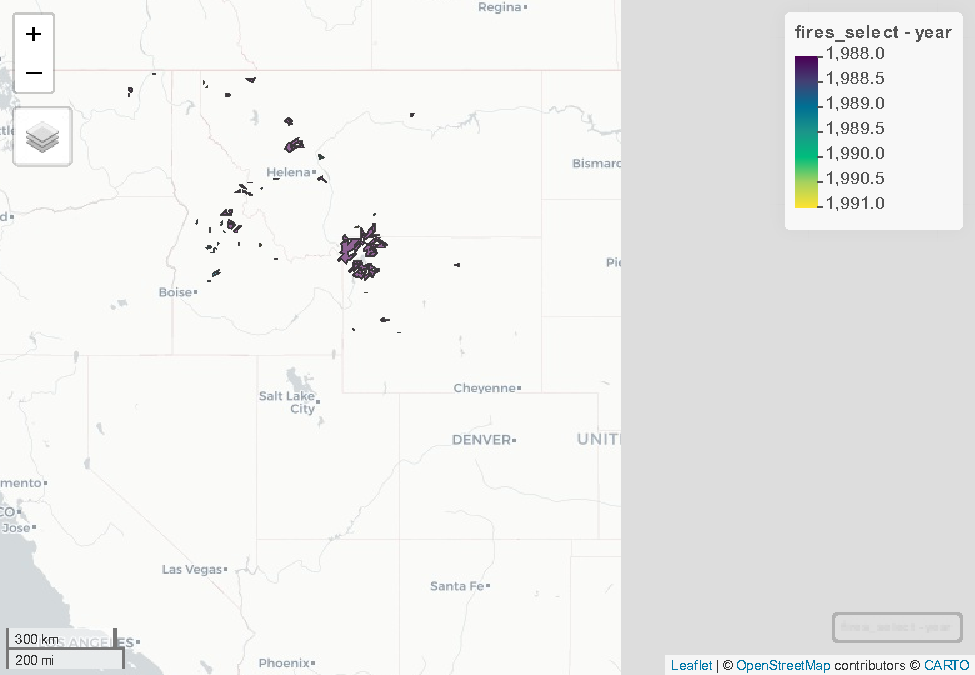
\includegraphics{_main_files/figure-latex/plot year-1.pdf}

\hypertarget{selected-fires-by-majority-forest-type}{%
\subsection{Selected fires by majority forest type}\label{selected-fires-by-majority-forest-type}}

\begin{Shaded}
\begin{Highlighting}[]
\CommentTok{\# plot}
\FunctionTok{mapview}\NormalTok{(fires\_select, }\AttributeTok{zcol =} \StringTok{"fire\_foresttype"}\NormalTok{)}
\end{Highlighting}
\end{Shaded}

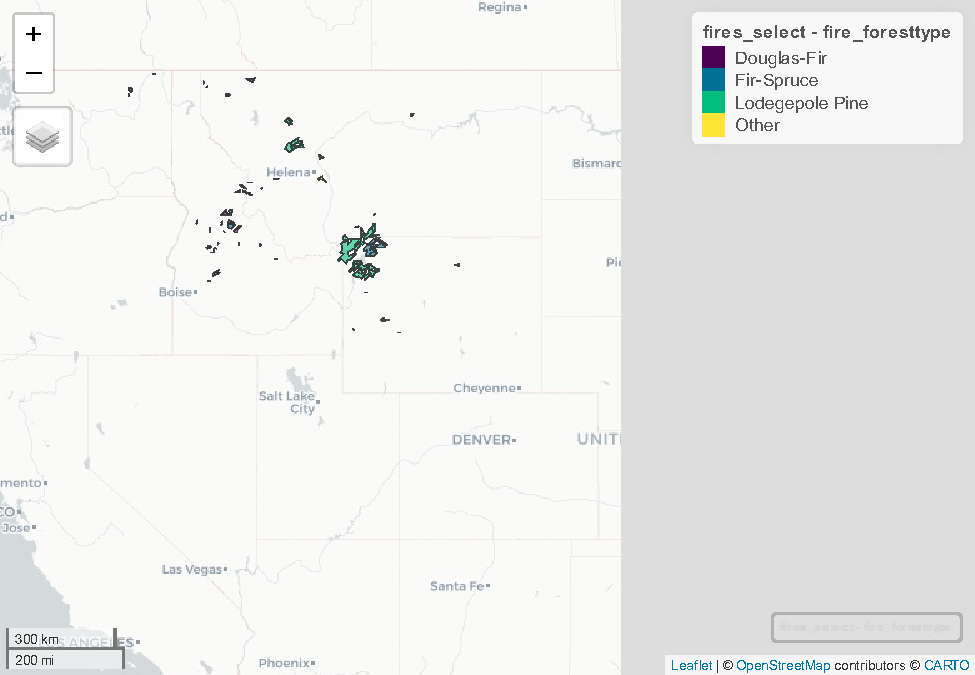
\includegraphics{_main_files/figure-latex/plot forest type-1.pdf}

\hypertarget{export-data}{%
\section{Export Data}\label{export-data}}

\hypertarget{final-cleanup-for-export}{%
\subsection{Final Cleanup for Export}\label{final-cleanup-for-export}}

\begin{Shaded}
\begin{Highlighting}[]
\CommentTok{\# reformat and project}
\NormalTok{fires\_export }\OtherTok{\textless{}{-}}\NormalTok{ fires\_select }\SpecialCharTok{\%\textgreater{}\%} 
  \FunctionTok{mutate}\NormalTok{(}\AttributeTok{year =} \FunctionTok{as.integer}\NormalTok{(year)) }\SpecialCharTok{\%\textgreater{}\%} 
  \FunctionTok{st\_transform}\NormalTok{(., }\AttributeTok{crs=}\StringTok{"EPSG:4326"}\NormalTok{)}

\NormalTok{mtbs\_export }\OtherTok{\textless{}{-}}\NormalTok{ fires\_mtbs }\SpecialCharTok{\%\textgreater{}\%} 
  \FunctionTok{mutate}\NormalTok{(}\AttributeTok{year =} \FunctionTok{as.integer}\NormalTok{(year)) }\SpecialCharTok{\%\textgreater{}\%} 
  \FunctionTok{st\_transform}\NormalTok{(., }\AttributeTok{crs=}\StringTok{"EPSG:4326"}\NormalTok{)}
\end{Highlighting}
\end{Shaded}

\hypertarget{export}{%
\subsection{Export}\label{export}}

\begin{Shaded}
\begin{Highlighting}[]
\CommentTok{\# st\_write(fires\_export, "data/fire\_boundaries/", "fires\_export.shp", driver = \textquotesingle{}ESRI Shapefile\textquotesingle{})}
\CommentTok{\# st\_write(mtbs\_export, "data/fire\_boundaries/", "mbts\_export.shp", driver = \textquotesingle{}ESRI Shapefile\textquotesingle{})}
\end{Highlighting}
\end{Shaded}

\hypertarget{patch-formation}{%
\chapter{Patch Formation}\label{patch-formation}}

\hypertarget{set-up-1}{%
\section{Set Up}\label{set-up-1}}

\hypertarget{libraries-1}{%
\subsection{Libraries}\label{libraries-1}}

\begin{Shaded}
\begin{Highlighting}[]
\FunctionTok{library}\NormalTok{(tidyverse)}
\FunctionTok{library}\NormalTok{(terra)}
\FunctionTok{library}\NormalTok{(patchwoRk)}
\FunctionTok{library}\NormalTok{(sf)}
\FunctionTok{library}\NormalTok{(mapview)}
\FunctionTok{library}\NormalTok{(exactextractr)}
\FunctionTok{library}\NormalTok{(lubridate)}
\end{Highlighting}
\end{Shaded}

\hypertarget{import-rdnbr-rasters}{%
\subsection{Import RdNBR Rasters}\label{import-rdnbr-rasters}}

\begin{Shaded}
\begin{Highlighting}[]
\CommentTok{\# import calculated RdNBR rasters for each fire boundary polygon}
\NormalTok{rast\_list }\OtherTok{\textless{}{-}} \FunctionTok{list.files}\NormalTok{(}\AttributeTok{path =} \StringTok{"data/rdnbr\_rasters"}\NormalTok{, }\AttributeTok{pattern=}\StringTok{\textquotesingle{}.tif\textquotesingle{}}\NormalTok{, }\AttributeTok{all.files=}\ConstantTok{TRUE}\NormalTok{, }\AttributeTok{full.names=}\ConstantTok{TRUE}\NormalTok{)}
\NormalTok{rast\_all }\OtherTok{\textless{}{-}} \FunctionTok{lapply}\NormalTok{(rast\_list, rast)}
\NormalTok{rast\_collection }\OtherTok{\textless{}{-}} \FunctionTok{sprc}\NormalTok{(rast\_all)}

\NormalTok{crs }\OtherTok{\textless{}{-}} \FunctionTok{crs}\NormalTok{(rast\_collection[}\DecValTok{1}\NormalTok{])}
\end{Highlighting}
\end{Shaded}

\hypertarget{import-fire-boundaries}{%
\subsection{Import Fire Boundaries}\label{import-fire-boundaries}}

\begin{Shaded}
\begin{Highlighting}[]
\CommentTok{\# import fire boundaries}
\NormalTok{mtbs\_export }\OtherTok{\textless{}{-}} \FunctionTok{st\_read}\NormalTok{(}\StringTok{\textquotesingle{}data/fire\_boundaries/mtbs\_export.shp\textquotesingle{}}\NormalTok{) }\SpecialCharTok{\%\textgreater{}\%} 
  \FunctionTok{st\_transform}\NormalTok{(., }\AttributeTok{crs=}\NormalTok{crs) }

\NormalTok{fires\_export }\OtherTok{\textless{}{-}} \FunctionTok{st\_read}\NormalTok{(}\StringTok{"data/fire\_boundaries/fires\_export.shp"}\NormalTok{)}\SpecialCharTok{\%\textgreater{}\%} 
  \FunctionTok{st\_transform}\NormalTok{(., }\AttributeTok{crs=}\NormalTok{crs)}

\CommentTok{\# import forest type group raster}
\NormalTok{conus\_forestgroup }\OtherTok{\textless{}{-}} \FunctionTok{raster}\NormalTok{(}\StringTok{\textquotesingle{}data/forest\_type/conus\_forestgroup.tif\textquotesingle{}}\NormalTok{)}
\NormalTok{forest\_codes }\OtherTok{\textless{}{-}} \FunctionTok{read\_csv}\NormalTok{(}\StringTok{\textquotesingle{}data/forest\_type/forestgroupcodes.csv\textquotesingle{}}\NormalTok{)}
\end{Highlighting}
\end{Shaded}

\hypertarget{create-high-severity-patches}{%
\section{Create High-Severity Patches}\label{create-high-severity-patches}}

\hypertarget{patchmorph}{%
\subsection{PatchMorph}\label{patchmorph}}

\begin{Shaded}
\begin{Highlighting}[]
\CommentTok{\# loop through RdNBR rasters, assign \textgreater{}640 to high severity category}
\CommentTok{\# utilize patchmorph to act as 3x3 cell majority filter}
\NormalTok{patch\_df }\OtherTok{\textless{}{-}} \FunctionTok{list}\NormalTok{()}
\ControlFlowTok{for}\NormalTok{ (i }\ControlFlowTok{in} \DecValTok{1}\SpecialCharTok{:}\FunctionTok{length}\NormalTok{(rast\_all))\{}
  \CommentTok{\# print(i)}
\NormalTok{  rast\_fire }\OtherTok{\textless{}{-}} \FunctionTok{raster}\NormalTok{(rast\_collection[i])}
\NormalTok{  rast\_fire[rast\_fire }\SpecialCharTok{\textless{}} \DecValTok{640}\NormalTok{] }\OtherTok{\textless{}{-}} \DecValTok{0}
\NormalTok{  rast\_fire[rast\_fire }\SpecialCharTok{\textgreater{}=} \DecValTok{640}\NormalTok{] }\OtherTok{\textless{}{-}} \DecValTok{1}

\NormalTok{  patch }\OtherTok{\textless{}{-}} \FunctionTok{patchMorph}\NormalTok{(rast\_fire, }\AttributeTok{spurThresh =} \DecValTok{3}\NormalTok{, }\AttributeTok{gapThresh =} \DecValTok{3}\NormalTok{)}
\NormalTok{  patch\_poly }\OtherTok{\textless{}{-}} \FunctionTok{as.polygons}\NormalTok{(}\FunctionTok{rast}\NormalTok{(patch)) }\SpecialCharTok{\%\textgreater{}\%}
    \FunctionTok{st\_as\_sf}\NormalTok{()}
\NormalTok{  df\_union\_cast }\OtherTok{\textless{}{-}}\NormalTok{ patch\_poly }\SpecialCharTok{\%\textgreater{}\%}
    \FunctionTok{st\_cast}\NormalTok{(., }\StringTok{"POLYGON"}\NormalTok{) }\SpecialCharTok{\%\textgreater{}\%}
    \FunctionTok{filter}\NormalTok{(layer }\SpecialCharTok{==} \DecValTok{1}\NormalTok{)}
\NormalTok{  patch\_df[[i]] }\OtherTok{\textless{}{-}}\NormalTok{ df\_union\_cast\}}

\NormalTok{patch\_poly\_all }\OtherTok{\textless{}{-}} \FunctionTok{do.call}\NormalTok{(rbind,patch\_df)}
\end{Highlighting}
\end{Shaded}

\hypertarget{refine-patches}{%
\section{Refine Patches}\label{refine-patches}}

\begin{Shaded}
\begin{Highlighting}[]
\CommentTok{\# filter small patches}
\NormalTok{patches\_full }\OtherTok{\textless{}{-}}\NormalTok{ patch\_poly\_all }\SpecialCharTok{\%\textgreater{}\%} 
  \FunctionTok{mutate}\NormalTok{(}\AttributeTok{patch\_area\_ha =} \FunctionTok{as.numeric}\NormalTok{(}\FunctionTok{st\_area}\NormalTok{(.))}\SpecialCharTok{/}\DecValTok{10000}\NormalTok{) }\SpecialCharTok{\%\textgreater{}\%}
  \FunctionTok{filter}\NormalTok{(patch\_area\_ha }\SpecialCharTok{\textgreater{}} \FloatTok{2.25}\NormalTok{)}
\end{Highlighting}
\end{Shaded}

\begin{Shaded}
\begin{Highlighting}[]
\CommentTok{\# join patches back to grouped fires}
\NormalTok{patches\_joined }\OtherTok{\textless{}{-}} \FunctionTok{st\_join}\NormalTok{(patches\_full,mtbs\_export,}\AttributeTok{join =}\NormalTok{ st\_intersects,}\AttributeTok{left=} \ConstantTok{FALSE}\NormalTok{,}\AttributeTok{largest =} \ConstantTok{TRUE}\NormalTok{) }\SpecialCharTok{\%\textgreater{}\%}
\NormalTok{  dplyr}\SpecialCharTok{::}\FunctionTok{select}\NormalTok{(}\SpecialCharTok{{-}}\NormalTok{layer,}\SpecialCharTok{{-}}\NormalTok{BurnBndAc) }\SpecialCharTok{\%\textgreater{}\%} 
  \FunctionTok{left\_join}\NormalTok{(.,}\FunctionTok{exact\_extract}\NormalTok{(conus\_forestgroup,., }\StringTok{\textquotesingle{}mode\textquotesingle{}}\NormalTok{, }\AttributeTok{append\_cols =} \ConstantTok{TRUE}\NormalTok{, }\AttributeTok{max\_cells\_in\_memory =} \FloatTok{3e+08}\NormalTok{))}\SpecialCharTok{\%\textgreater{}\%}
  \FunctionTok{mutate}\NormalTok{(}\AttributeTok{patch\_foresttype =} \FunctionTok{case\_when}\NormalTok{(mode}\SpecialCharTok{==}\DecValTok{200} \SpecialCharTok{\textasciitilde{}} \StringTok{"Douglas{-}Fir"}\NormalTok{,}
\NormalTok{                                     mode}\SpecialCharTok{==}\DecValTok{220} \SpecialCharTok{\textasciitilde{}} \StringTok{"Ponderosa"}\NormalTok{,}
\NormalTok{                                     mode}\SpecialCharTok{==}\DecValTok{260} \SpecialCharTok{\textasciitilde{}} \StringTok{"Fir{-}Spruce"}\NormalTok{,}
\NormalTok{                                     mode}\SpecialCharTok{==}\DecValTok{280} \SpecialCharTok{\textasciitilde{}} \StringTok{"Lodegepole Pine"}\NormalTok{,}
\NormalTok{                                     mode}\SpecialCharTok{==}\DecValTok{0} \SpecialCharTok{\textasciitilde{}} \StringTok{"Unforested"}\NormalTok{,}
                                     \ConstantTok{TRUE} \SpecialCharTok{\textasciitilde{}} \StringTok{"Other"}\NormalTok{))}
\end{Highlighting}
\end{Shaded}

\hypertarget{mapping-1}{%
\section{Mapping}\label{mapping-1}}

\begin{Shaded}
\begin{Highlighting}[]
\FunctionTok{mapview}\NormalTok{(patches\_joined,}\AttributeTok{col.regions =} \StringTok{"red"}\NormalTok{) }\SpecialCharTok{+} \FunctionTok{mapview}\NormalTok{(fires\_export, }\AttributeTok{alpha.regions =} \DecValTok{0}\NormalTok{, }\AttributeTok{lwd =} \DecValTok{2}\NormalTok{)}
\end{Highlighting}
\end{Shaded}

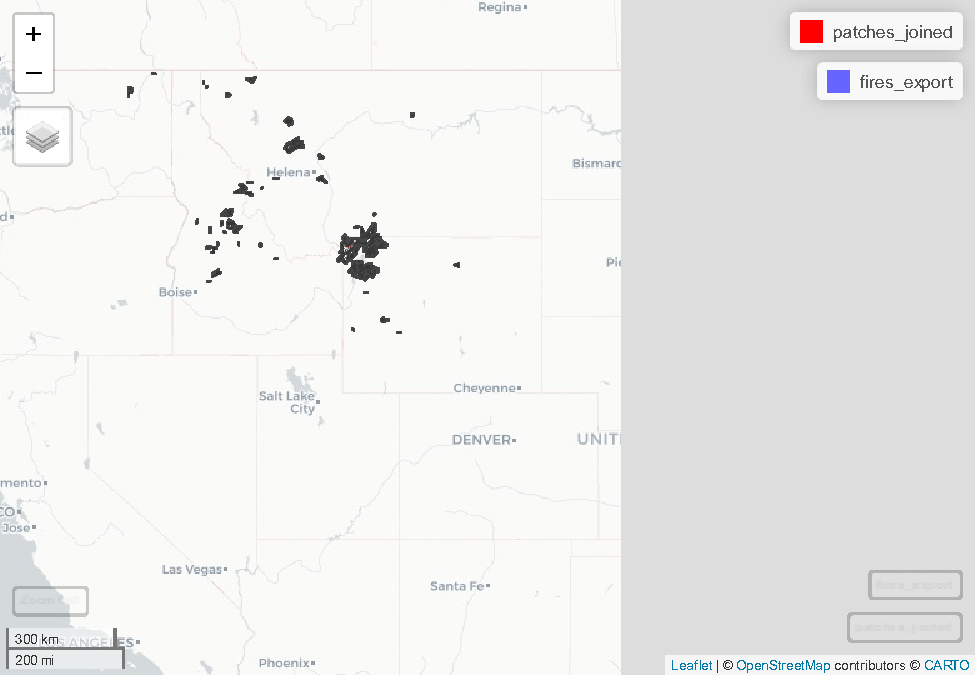
\includegraphics{_main_files/figure-latex/map-1.pdf}

\hypertarget{export-data-1}{%
\section{Export Data}\label{export-data-1}}

\begin{Shaded}
\begin{Highlighting}[]
\NormalTok{patches }\OtherTok{\textless{}{-}}\NormalTok{ patches\_joined }\SpecialCharTok{\%\textgreater{}\%}
  \FunctionTok{st\_transform}\NormalTok{(}\AttributeTok{crs =}\NormalTok{ crs)}

\CommentTok{\# st\_write(patches, "data/patches/", "highsev\_patches.shp",driver = \textquotesingle{}ESRI Shapefile\textquotesingle{})}
\end{Highlighting}
\end{Shaded}

\hypertarget{sampling-quadrants}{%
\chapter{Sampling Quadrants}\label{sampling-quadrants}}

\hypertarget{set-up-2}{%
\section{Set Up}\label{set-up-2}}

\hypertarget{libraries-2}{%
\subsection{Libraries}\label{libraries-2}}

\begin{Shaded}
\begin{Highlighting}[]
\FunctionTok{library}\NormalTok{(elevatr)}
\FunctionTok{library}\NormalTok{(tidyverse)}
\FunctionTok{library}\NormalTok{(sf)}
\FunctionTok{library}\NormalTok{(terra)}
\FunctionTok{library}\NormalTok{(mapview)}
\end{Highlighting}
\end{Shaded}

\hypertarget{import-high-severity-patches-and-fire-boundaries}{%
\subsection{Import High-Severity Patches and Fire Boundaries}\label{import-high-severity-patches-and-fire-boundaries}}

\begin{Shaded}
\begin{Highlighting}[]
\CommentTok{\# data import}
\NormalTok{patches }\OtherTok{\textless{}{-}} \FunctionTok{st\_read}\NormalTok{(}\StringTok{"data/patches/highsev\_patches.shp"}\NormalTok{) }\SpecialCharTok{\%\textgreater{}\%} 
  \FunctionTok{st\_transform}\NormalTok{(}\AttributeTok{crs=}\StringTok{"EPSG:4326"}\NormalTok{)}
\NormalTok{crs }\OtherTok{\textless{}{-}} \FunctionTok{crs}\NormalTok{(patches)}

\NormalTok{patch\_interiors}\OtherTok{\textless{}{-}} \FunctionTok{st\_read}\NormalTok{(}\StringTok{"data/patches/highsev\_patches\_interior.shp"}\NormalTok{) }\SpecialCharTok{\%\textgreater{}\%}
  \FunctionTok{st\_transform}\NormalTok{(}\AttributeTok{crs=}\NormalTok{crs)}
\NormalTok{patch\_exteriors}\OtherTok{\textless{}{-}} \FunctionTok{st\_read}\NormalTok{(}\StringTok{"data/patches/highsev\_patches\_exterior.shp"}\NormalTok{) }\SpecialCharTok{\%\textgreater{}\%}
  \FunctionTok{st\_transform}\NormalTok{(}\AttributeTok{crs=}\NormalTok{crs)}

\NormalTok{mtbs\_export }\OtherTok{\textless{}{-}} \FunctionTok{st\_read}\NormalTok{(}\StringTok{\textquotesingle{}data/fire\_boundaries/mtbs\_export.shp\textquotesingle{}}\NormalTok{) }\SpecialCharTok{\%\textgreater{}\%} 
  \FunctionTok{st\_transform}\NormalTok{(}\AttributeTok{crs=}\NormalTok{crs) }

\NormalTok{fires\_export }\OtherTok{\textless{}{-}} \FunctionTok{st\_read}\NormalTok{(}\StringTok{"data/fire\_boundaries/fires\_export.shp"}\NormalTok{)}\SpecialCharTok{\%\textgreater{}\%} 
  \FunctionTok{st\_transform}\NormalTok{(}\AttributeTok{crs=}\NormalTok{crs)}
\end{Highlighting}
\end{Shaded}

\hypertarget{create-sampling-quadrants}{%
\section{Create Sampling Quadrants}\label{create-sampling-quadrants}}

\hypertarget{split-patches-by-northsouth-aspects-and-interiorexterior}{%
\subsection{Split Patches by North/South Aspects and Interior/Exterior}\label{split-patches-by-northsouth-aspects-and-interiorexterior}}

\begin{Shaded}
\begin{Highlighting}[]
\CommentTok{\# create list of fire IDs}
\NormalTok{fire\_list }\OtherTok{\textless{}{-}} \FunctionTok{unique}\NormalTok{(patches}\SpecialCharTok{$}\NormalTok{Evnt\_ID)}

\NormalTok{quadrants\_df }\OtherTok{=} \FunctionTok{list}\NormalTok{()}

\ControlFlowTok{for}\NormalTok{(i }\ControlFlowTok{in}\NormalTok{ fire\_list)\{}
  
  \CommentTok{\# filter patch interiors/exteriors to the selected fire}
\NormalTok{  patch\_fire }\OtherTok{\textless{}{-}}\NormalTok{ patches }\SpecialCharTok{\%\textgreater{}\%} 
    \FunctionTok{filter}\NormalTok{(Evnt\_ID }\SpecialCharTok{==}\NormalTok{ i)}
  
  \FunctionTok{mapview}\NormalTok{(patch\_fire)}
  
\NormalTok{  patches\_interior }\OtherTok{\textless{}{-}}\NormalTok{ patch\_interiors }\SpecialCharTok{\%\textgreater{}\%} 
    \FunctionTok{filter}\NormalTok{(Evnt\_ID }\SpecialCharTok{==}\NormalTok{ i)}\SpecialCharTok{\%\textgreater{}\%} 
    \FunctionTok{st\_make\_valid}\NormalTok{() }\SpecialCharTok{\%\textgreater{}\%} 
    \FunctionTok{st\_union}\NormalTok{()}
  
\NormalTok{  patches\_exterior }\OtherTok{\textless{}{-}}\NormalTok{ patch\_exteriors }\SpecialCharTok{\%\textgreater{}\%} 
    \FunctionTok{filter}\NormalTok{(Evnt\_ID\_1 }\SpecialCharTok{==}\NormalTok{ i)}\SpecialCharTok{\%\textgreater{}\%} 
    \FunctionTok{st\_make\_valid}\NormalTok{()}\SpecialCharTok{\%\textgreater{}\%} 
    \FunctionTok{st\_union}\NormalTok{()}
  
  \CommentTok{\# set event and fire id to the selected fire}
\NormalTok{  Evnt\_ID }\OtherTok{\textless{}{-}}\NormalTok{ i}
\NormalTok{  Fire\_ID }\OtherTok{\textless{}{-}}\FunctionTok{names}\NormalTok{(}\FunctionTok{which.max}\NormalTok{(}\FunctionTok{table}\NormalTok{(patch\_fire}\SpecialCharTok{$}\NormalTok{Fire\_ID)))}
  
  \FunctionTok{print}\NormalTok{(}\FunctionTok{paste0}\NormalTok{(}\StringTok{"starting event "}\NormalTok{,Evnt\_ID,}\StringTok{" in fire group "}\NormalTok{, Fire\_ID))}
  
  \CommentTok{\# get and calculate cosine corrected aspect}
\NormalTok{  dem }\OtherTok{\textless{}{-}} \FunctionTok{get\_elev\_raster}\NormalTok{(patch\_fire,}\AttributeTok{z=}\DecValTok{11}\NormalTok{)}
\NormalTok{  aspect }\OtherTok{\textless{}{-}} \FunctionTok{terrain}\NormalTok{(dem, }\AttributeTok{opt =} \StringTok{"aspect"}\NormalTok{,}\AttributeTok{unit =} \StringTok{"radians"}\NormalTok{)}
\NormalTok{  ccaspect }\OtherTok{\textless{}{-}} \FunctionTok{cos}\NormalTok{(aspect)}

  \CommentTok{\# positive aspects are north{-}facing, negative are south{-}facing}
\NormalTok{  ccaspect[ccaspect}\SpecialCharTok{\textgreater{}}\DecValTok{0}\NormalTok{] }\OtherTok{\textless{}{-}} \DecValTok{1}
\NormalTok{  ccaspect[ccaspect}\SpecialCharTok{\textless{}}\DecValTok{0}\NormalTok{] }\OtherTok{\textless{}{-}} \SpecialCharTok{{-}}\DecValTok{1}
\NormalTok{  ccaspect\_poly }\OtherTok{\textless{}{-}} \FunctionTok{as.polygons}\NormalTok{(}\FunctionTok{rast}\NormalTok{(ccaspect)) }\SpecialCharTok{\%\textgreater{}\%}
    \FunctionTok{st\_as\_sf}\NormalTok{()}
  
\NormalTok{  pos\_aspect }\OtherTok{\textless{}{-}}\NormalTok{ ccaspect\_poly }\SpecialCharTok{\%\textgreater{}\%}
    \FunctionTok{filter}\NormalTok{(layer}\SpecialCharTok{==}\DecValTok{1}\NormalTok{)}\SpecialCharTok{\%\textgreater{}\%} 
    \FunctionTok{st\_make\_valid}\NormalTok{()}
\NormalTok{  neg\_aspect }\OtherTok{\textless{}{-}}\NormalTok{ ccaspect\_poly }\SpecialCharTok{\%\textgreater{}\%}
    \FunctionTok{filter}\NormalTok{(layer}\SpecialCharTok{=={-}}\DecValTok{1}\NormalTok{) }\SpecialCharTok{\%\textgreater{}\%} 
    \FunctionTok{st\_make\_valid}\NormalTok{()}

  \CommentTok{\# get quadrants as the intersection of interior/exterior and pos/neg aspect}
\NormalTok{  pos\_ext }\OtherTok{\textless{}{-}} \FunctionTok{st\_intersection}\NormalTok{(patches\_exterior,pos\_aspect)}\SpecialCharTok{\%\textgreater{}\%} 
    \FunctionTok{st\_make\_valid}\NormalTok{() }\SpecialCharTok{\%\textgreater{}\%} 
    \FunctionTok{st\_union}\NormalTok{() }\SpecialCharTok{\%\textgreater{}\%} 
    \FunctionTok{st\_as\_sf}\NormalTok{()}\SpecialCharTok{\%\textgreater{}\%} 
    \FunctionTok{mutate}\NormalTok{(}\AttributeTok{quadrant =} \StringTok{"pos\_ext"}\NormalTok{,}
           \AttributeTok{Evnt\_ID =}\NormalTok{ i,}
           \AttributeTok{quad\_id\_event =} \FunctionTok{paste0}\NormalTok{(Evnt\_ID,}\StringTok{"{-}"}\NormalTok{,quadrant),}
           \AttributeTok{Fire\_ID =}\NormalTok{ Fire\_ID,}
           \AttributeTok{quad\_id\_fire =} \FunctionTok{paste0}\NormalTok{(Fire\_ID,}\StringTok{"{-}"}\NormalTok{,quadrant))}

\NormalTok{  pos\_int }\OtherTok{\textless{}{-}} \FunctionTok{st\_intersection}\NormalTok{(patches\_interior,pos\_aspect)}\SpecialCharTok{\%\textgreater{}\%} 
    \FunctionTok{st\_make\_valid}\NormalTok{() }\SpecialCharTok{\%\textgreater{}\%} 
    \FunctionTok{st\_union}\NormalTok{()}\SpecialCharTok{\%\textgreater{}\%} 
    \FunctionTok{st\_as\_sf}\NormalTok{()}\SpecialCharTok{\%\textgreater{}\%} 
    \FunctionTok{mutate}\NormalTok{(}\AttributeTok{quadrant =} \StringTok{"pos\_int"}\NormalTok{,}
           \AttributeTok{Evnt\_ID =}\NormalTok{ i,}
           \AttributeTok{quad\_id\_event =} \FunctionTok{paste0}\NormalTok{(Evnt\_ID,}\StringTok{"{-}"}\NormalTok{,quadrant),}
           \AttributeTok{Fire\_ID =}\NormalTok{ Fire\_ID,}
           \AttributeTok{quad\_id\_fire =} \FunctionTok{paste0}\NormalTok{(Fire\_ID,}\StringTok{"{-}"}\NormalTok{,quadrant))}
  
\NormalTok{  neg\_ext }\OtherTok{\textless{}{-}} \FunctionTok{st\_intersection}\NormalTok{(patches\_exterior,neg\_aspect)}\SpecialCharTok{\%\textgreater{}\%} 
    \FunctionTok{st\_make\_valid}\NormalTok{() }\SpecialCharTok{\%\textgreater{}\%}
    \FunctionTok{st\_union}\NormalTok{() }\SpecialCharTok{\%\textgreater{}\%} 
    \FunctionTok{st\_as\_sf}\NormalTok{()}\SpecialCharTok{\%\textgreater{}\%} 
    \FunctionTok{mutate}\NormalTok{(}\AttributeTok{quadrant =} \StringTok{"neg\_ext"}\NormalTok{,}
           \AttributeTok{Evnt\_ID =}\NormalTok{ i,}
           \AttributeTok{quad\_id\_event =} \FunctionTok{paste0}\NormalTok{(Evnt\_ID,}\StringTok{"{-}"}\NormalTok{,quadrant),}
           \AttributeTok{Fire\_ID =}\NormalTok{ Fire\_ID,}
           \AttributeTok{quad\_id\_fire =} \FunctionTok{paste0}\NormalTok{(Fire\_ID,}\StringTok{"{-}"}\NormalTok{,quadrant))}
  
\NormalTok{  neg\_int }\OtherTok{\textless{}{-}} \FunctionTok{st\_intersection}\NormalTok{(patches\_interior, neg\_aspect)}\SpecialCharTok{\%\textgreater{}\%} 
    \FunctionTok{st\_make\_valid}\NormalTok{() }\SpecialCharTok{\%\textgreater{}\%}
    \FunctionTok{st\_union}\NormalTok{() }\SpecialCharTok{\%\textgreater{}\%} 
    \FunctionTok{st\_as\_sf}\NormalTok{()}\SpecialCharTok{\%\textgreater{}\%} 
    \FunctionTok{mutate}\NormalTok{(}\AttributeTok{quadrant =} \StringTok{"neg\_int"}\NormalTok{,}
           \AttributeTok{Evnt\_ID =}\NormalTok{ i,}
           \AttributeTok{quad\_id\_event =} \FunctionTok{paste0}\NormalTok{(Evnt\_ID,}\StringTok{"{-}"}\NormalTok{,quadrant),}
           \AttributeTok{Fire\_ID =}\NormalTok{ Fire\_ID,}
           \AttributeTok{quad\_id\_fire =} \FunctionTok{paste0}\NormalTok{(Fire\_ID,}\StringTok{"{-}"}\NormalTok{,quadrant))}
  
  \CommentTok{\# combine, export quadrants}
\NormalTok{  all\_quadrants }\OtherTok{\textless{}{-}} \FunctionTok{rbind}\NormalTok{(neg\_int,pos\_int,neg\_ext,pos\_ext) }\SpecialCharTok{\%\textgreater{}\%} 
    \FunctionTok{st\_transform}\NormalTok{(}\AttributeTok{crs=}\NormalTok{crs)}

\NormalTok{  quadrants\_df[[i]] }\OtherTok{\textless{}{-}}\NormalTok{ all\_quadrants}
  
  \FunctionTok{print}\NormalTok{(}\FunctionTok{paste0}\NormalTok{(}\StringTok{"completed"}\NormalTok{))}
\NormalTok{\}}

\CommentTok{\# bind list together}
\NormalTok{quadrants\_fullset }\OtherTok{\textless{}{-}} \FunctionTok{do.call}\NormalTok{(rbind,quadrants\_df) }\SpecialCharTok{\%\textgreater{}\%} 
  \FunctionTok{st\_as\_sf}\NormalTok{() }
\end{Highlighting}
\end{Shaded}

\hypertarget{clean-quadrants}{%
\subsection{Clean Quadrants}\label{clean-quadrants}}

\begin{Shaded}
\begin{Highlighting}[]
\CommentTok{\# removes erroneous polygons created from irregular fire boundary shapes}
\CommentTok{\# removes small border mismatched fire}
\NormalTok{quadrants\_clean }\OtherTok{\textless{}{-}}\NormalTok{ quadrants\_fullset }\SpecialCharTok{\%\textgreater{}\%} 
  \FunctionTok{mutate}\NormalTok{(}\AttributeTok{area=}\FunctionTok{as.numeric}\NormalTok{(}\FunctionTok{st\_area}\NormalTok{(x))) }\SpecialCharTok{\%\textgreater{}\%} 
  \FunctionTok{filter}\NormalTok{(area }\SpecialCharTok{\textgreater{}} \DecValTok{1}\NormalTok{) }\SpecialCharTok{\%\textgreater{}\%} 
  \FunctionTok{group\_by}\NormalTok{(Evnt\_ID) }\SpecialCharTok{\%\textgreater{}\%} 
  \FunctionTok{mutate}\NormalTok{(}\AttributeTok{n=}\FunctionTok{n}\NormalTok{()) }\SpecialCharTok{\%\textgreater{}\%} 
  \FunctionTok{filter}\NormalTok{(n }\SpecialCharTok{==} \DecValTok{4}\NormalTok{)}

\CommentTok{\# clean up for export}
\NormalTok{quadrants\_export }\OtherTok{\textless{}{-}}\NormalTok{ quadrants\_clean }\SpecialCharTok{\%\textgreater{}\%} 
  \FunctionTok{st\_make\_valid}\NormalTok{() }\SpecialCharTok{\%\textgreater{}\%} 
  \FunctionTok{st\_as\_sf}\NormalTok{() }\SpecialCharTok{\%\textgreater{}\%} 
\NormalTok{  dplyr}\SpecialCharTok{::}\FunctionTok{select}\NormalTok{(}\SpecialCharTok{{-}}\StringTok{"area"}\NormalTok{)}\SpecialCharTok{\%\textgreater{}\%} 
  \FunctionTok{st\_transform}\NormalTok{(}\AttributeTok{crs=}\NormalTok{crs)}
\end{Highlighting}
\end{Shaded}

\hypertarget{export-data-2}{%
\section{Export Data}\label{export-data-2}}

\begin{Shaded}
\begin{Highlighting}[]
\CommentTok{\# st\_write(quadrants\_export,"data/patches/","quadrants\_export.shp",driver = "ESRI Shapefile")}
\end{Highlighting}
\end{Shaded}

\hypertarget{training-data}{%
\chapter{Training Data}\label{training-data}}

\hypertarget{set-up-3}{%
\section{Set Up}\label{set-up-3}}

\hypertarget{libraries-3}{%
\subsubsection{Libraries}\label{libraries-3}}

\begin{Shaded}
\begin{Highlighting}[]
\FunctionTok{library}\NormalTok{(tidyverse)}
\FunctionTok{library}\NormalTok{(sf)}
\FunctionTok{library}\NormalTok{(terra)}
\end{Highlighting}
\end{Shaded}

\hypertarget{import-data}{%
\section{Import Data}\label{import-data}}

\begin{Shaded}
\begin{Highlighting}[]
\NormalTok{patches }\OtherTok{\textless{}{-}} \FunctionTok{st\_read}\NormalTok{(}\StringTok{"data/patches/highsev\_patches.shp"}\NormalTok{) }\SpecialCharTok{\%\textgreater{}\%} 
  \FunctionTok{st\_transform}\NormalTok{(}\AttributeTok{crs=}\StringTok{"EPSG: 4326"}\NormalTok{)}

\NormalTok{crs }\OtherTok{\textless{}{-}} \FunctionTok{crs}\NormalTok{(patches)}

\NormalTok{quadrants }\OtherTok{\textless{}{-}} \FunctionTok{st\_read}\NormalTok{(}\StringTok{"data/patches/quadrants\_export.shp"}\NormalTok{) }\SpecialCharTok{\%\textgreater{}\%} 
  \FunctionTok{st\_transform}\NormalTok{(}\AttributeTok{crs=}\NormalTok{crs)}
\end{Highlighting}
\end{Shaded}

\hypertarget{sampling-points}{%
\section{Sampling Points}\label{sampling-points}}

\hypertarget{import-and-combine-training-points}{%
\subsection{Import and Combine Training Points}\label{import-and-combine-training-points}}

\begin{Shaded}
\begin{Highlighting}[]
\NormalTok{points\_list }\OtherTok{\textless{}{-}} \FunctionTok{list.files}\NormalTok{(}\AttributeTok{path =} \StringTok{"data/points/individual\_fire\_points/"}\NormalTok{, }\AttributeTok{pattern=}\StringTok{\textquotesingle{}.shp\textquotesingle{}}\NormalTok{, }\AttributeTok{all.files=}\ConstantTok{TRUE}\NormalTok{, }\AttributeTok{full.names=}\ConstantTok{TRUE}\NormalTok{)}
\NormalTok{points\_all }\OtherTok{\textless{}{-}} \FunctionTok{lapply}\NormalTok{(points\_list, st\_read)}

\NormalTok{points }\OtherTok{\textless{}{-}} \FunctionTok{do.call}\NormalTok{(rbind,points\_all) }\SpecialCharTok{\%\textgreater{}\%} 
  \FunctionTok{st\_transform}\NormalTok{(}\AttributeTok{crs=}\NormalTok{crs)}
\end{Highlighting}
\end{Shaded}

\hypertarget{assign-points-and-clean-data}{%
\subsection{Assign Points and Clean Data}\label{assign-points-and-clean-data}}

\begin{Shaded}
\begin{Highlighting}[]
\CommentTok{\# join points dataset back to fires to fill out dataset}
\NormalTok{points\_joined }\OtherTok{\textless{}{-}} \FunctionTok{st\_join}\NormalTok{(points,patches,}\AttributeTok{left=}\ConstantTok{TRUE}\NormalTok{,}\AttributeTok{largest=}\ConstantTok{TRUE}\NormalTok{) }\SpecialCharTok{\%\textgreater{}\%} 
  \FunctionTok{st\_join}\NormalTok{(.,quadrants,}\AttributeTok{left=}\ConstantTok{TRUE}\NormalTok{,}\AttributeTok{largest=}\ConstantTok{TRUE}\NormalTok{)}
\end{Highlighting}
\end{Shaded}

\begin{verbatim}
## Warning: attribute variables are assumed to be spatially constant throughout all
## geometries

## Warning: attribute variables are assumed to be spatially constant throughout all
## geometries
\end{verbatim}

\begin{Shaded}
\begin{Highlighting}[]
\NormalTok{points\_cleaned }\OtherTok{\textless{}{-}}\NormalTok{ points\_joined }\SpecialCharTok{\%\textgreater{}\%} 
\NormalTok{  dplyr}\SpecialCharTok{::}\FunctionTok{select}\NormalTok{(}\StringTok{"class"}\NormalTok{,}\StringTok{"ptch\_r\_"}\NormalTok{,}\StringTok{"Evnt\_ID.x"}\NormalTok{,}\StringTok{"Incd\_Nm"}\NormalTok{,}\StringTok{"Fire\_ID.x"}\NormalTok{,}\StringTok{"year"}\NormalTok{,}\StringTok{"ecoregn"}\NormalTok{,}\StringTok{"ptch\_fr"}\NormalTok{,}\StringTok{"quadrnt"}\NormalTok{,}\StringTok{"qd\_d\_vn"}\NormalTok{,}\StringTok{"qd\_d\_fr"}\NormalTok{) }\SpecialCharTok{\%\textgreater{}\%} 
  \FunctionTok{rename}\NormalTok{(}\AttributeTok{patch\_area\_ha =}\NormalTok{ ptch\_r\_,}
         \AttributeTok{Event\_ID =}\NormalTok{ Evnt\_ID.x,}
         \AttributeTok{Incid\_Name =}\NormalTok{ Incd\_Nm,}
         \AttributeTok{Fire\_ID =}\NormalTok{ Fire\_ID.x,}
         \AttributeTok{patch\_frtype =}\NormalTok{ ptch\_fr,}
         \AttributeTok{quad =}\NormalTok{ quadrnt,}
         \AttributeTok{quad\_event\_id=}\NormalTok{ qd\_d\_vn,}
         \AttributeTok{quad\_fire\_id=}\NormalTok{qd\_d\_fr) }\SpecialCharTok{\%\textgreater{}\%} 
  \FunctionTok{st\_transform}\NormalTok{(}\AttributeTok{crs=}\NormalTok{crs)}
\end{Highlighting}
\end{Shaded}

\hypertarget{export-1}{%
\section{Export}\label{export-1}}

\begin{Shaded}
\begin{Highlighting}[]
\CommentTok{\# st\_write(points\_cleaned, "data/points/", "points\_export.shp",driver = \textquotesingle{}ESRI Shapefile\textquotesingle{})}
\end{Highlighting}
\end{Shaded}


  \bibliography{book.bib,packages.bib}

\end{document}
